\documentclass[]{article}
\usepackage{lmodern}
\usepackage{amssymb,amsmath}
\usepackage{ifxetex,ifluatex}
\usepackage{fixltx2e} % provides \textsubscript
\ifnum 0\ifxetex 1\fi\ifluatex 1\fi=0 % if pdftex
  \usepackage[T1]{fontenc}
  \usepackage[utf8]{inputenc}
\else % if luatex or xelatex
  \ifxetex
    \usepackage{mathspec}
  \else
    \usepackage{fontspec}
  \fi
  \defaultfontfeatures{Ligatures=TeX,Scale=MatchLowercase}
\fi
% use upquote if available, for straight quotes in verbatim environments
\IfFileExists{upquote.sty}{\usepackage{upquote}}{}
% use microtype if available
\IfFileExists{microtype.sty}{%
\usepackage{microtype}
\UseMicrotypeSet[protrusion]{basicmath} % disable protrusion for tt fonts
}{}
\usepackage[margin=1in]{geometry}
\usepackage{hyperref}
\hypersetup{unicode=true,
            pdftitle={Is malaria control profitable? Return on investment of privately-managed residential fumigations at a large sugarcane processing facility in Southern Mozambique},
            pdfborder={0 0 0},
            breaklinks=true}
\urlstyle{same}  % don't use monospace font for urls
\usepackage{graphicx,grffile}
\makeatletter
\def\maxwidth{\ifdim\Gin@nat@width>\linewidth\linewidth\else\Gin@nat@width\fi}
\def\maxheight{\ifdim\Gin@nat@height>\textheight\textheight\else\Gin@nat@height\fi}
\makeatother
% Scale images if necessary, so that they will not overflow the page
% margins by default, and it is still possible to overwrite the defaults
% using explicit options in \includegraphics[width, height, ...]{}
\setkeys{Gin}{width=\maxwidth,height=\maxheight,keepaspectratio}
\IfFileExists{parskip.sty}{%
\usepackage{parskip}
}{% else
\setlength{\parindent}{0pt}
\setlength{\parskip}{6pt plus 2pt minus 1pt}
}
\setlength{\emergencystretch}{3em}  % prevent overfull lines
\providecommand{\tightlist}{%
  \setlength{\itemsep}{0pt}\setlength{\parskip}{0pt}}
\setcounter{secnumdepth}{0}
% Redefines (sub)paragraphs to behave more like sections
\ifx\paragraph\undefined\else
\let\oldparagraph\paragraph
\renewcommand{\paragraph}[1]{\oldparagraph{#1}\mbox{}}
\fi
\ifx\subparagraph\undefined\else
\let\oldsubparagraph\subparagraph
\renewcommand{\subparagraph}[1]{\oldsubparagraph{#1}\mbox{}}
\fi

%%% Use protect on footnotes to avoid problems with footnotes in titles
\let\rmarkdownfootnote\footnote%
\def\footnote{\protect\rmarkdownfootnote}

%%% Change title format to be more compact
\usepackage{titling}

% Create subtitle command for use in maketitle
\newcommand{\subtitle}[1]{
  \posttitle{
    \begin{center}\large#1\end{center}
    }
}

\setlength{\droptitle}{-2em}
  \title{Is malaria control profitable? Return on investment of privately-managed
residential fumigations at a large sugarcane processing facility in
Southern Mozambique}
  \pretitle{\vspace{\droptitle}\centering\huge}
  \posttitle{\par}
  \author{}
  \preauthor{}\postauthor{}
  \date{}
  \predate{}\postdate{}

\pagenumbering{gobble}
\usepackage{longtable}
\usepackage[utf8]{inputenc}
\usepackage{changepage}
\usepackage{graphicx}
\usepackage{multicol}
\usepackage{geometry}
\usepackage{fancyhdr}
\usepackage{color}
\usepackage{colortbl}
\usepackage{color}
% Font
\usepackage{fontspec}
\setmainfont{Swift-Regular_43151.ttf}
\setsansfont[BoldFont={Swift-Bold_43130.ttf}]{Swift-Regular_43151.ttf}
% \setmonofont{Swift-Regular_43151.ttf}
\renewcommand{\familydefault}{\sfdefault}
% \usepackage{fontspec}
% \setmainfont{Lato-Regular.ttf}
% \setsansfont[BoldFont={Lato-Bold.ttf}]{Lato-Regular.ttf}
% \renewcommand{\familydefault}{\sfdefault}

\def\changemargin#1#2{\list{}{\rightmargin#2\leftmargin#1}\item[]}
\let\endchangemargin=\endlist
\renewcommand{\rmdefault}{ppl}

\usepackage{multicol}
\usepackage{hyperref}
\usepackage{geometry}
\usepackage{lipsum}

\usepackage{float}
\floatplacement{figure}{H}

% \usepackage{todonotes} % for side notes
% \usepackage[colorinlistoftodos]{todonotes} % for side notes

\usepackage{xargs}                      % Use more than one optional parameter in a new commands
\usepackage[dvipsnames, table]{xcolor}  % Coloured text etc.
% 
\usepackage[colorinlistoftodos,prependcaption,textsize=tiny]{todonotes}
\newcommandx{\unsure}[2][1=]{\todo[linecolor=red,backgroundcolor=red!25,bordercolor=red,#1]{#2}}
\newcommandx{\change}[2][1=]{\todo[linecolor=blue,backgroundcolor=blue!25,bordercolor=blue,#1]{#2}}
\newcommandx{\info}[2][1=]{\todo[linecolor=OliveGreen,backgroundcolor=OliveGreen!25,bordercolor=OliveGreen,#1]{#2}}
\newcommandx{\improvement}[2][1=]{\todo[linecolor=Plum,backgroundcolor=Plum!25,bordercolor=Plum,#1]{#2}}
\newcommandx{\thiswillnotshow}[2][1=]{\todo[disable,#1]{#2}}
\usepackage{lmodern}
\usepackage{fancyhdr} % Headers and footers
\pagestyle{fancy} % All pages have headers and footers
\fancyhead{} % Blank out the default header
\fancyfoot{} % Blank out the default footer
\fancyhead[C]{Return on investment of private sector malaria control at a large sugar facility in Southern Mozambique}
\renewcommand{\thefootnote}{\fnsymbol{footnote}}

\newcommand{\footremember}[2]{%
    \footnote{#2}
    \newcounter{#1}
    \setcounter{#1}{\value{footnote}}%
}
\newcommand{\footrecall}[1]{%
    \footnotemark[\value{#1}]%
}

\def\changemargin#1#2{\list{}{\rightmargin#2\leftmargin#1}\item[]}
\let\endchangemargin=\endlist

\widowpenalties 1 150

\makeatletter
\renewcommand\footnotesize{%
   \@setfontsize\footnotesize\@ixpt{11}%
   \abovedisplayskip 8\p@ \@plus2\p@ \@minus4\p@
   \abovedisplayshortskip \z@ \@plus\p@
   \belowdisplayshortskip 4\p@ \@plus2\p@ \@minus2\p@
   \def\@listi{\leftmargin\leftmargini
               \topsep 4\p@ \@plus2\p@ \@minus2\p@
               \parsep 2\p@ \@plus\p@ \@minus\p@
               \itemsep \parsep}%
   \belowdisplayskip \abovedisplayskip
}
\makeatother

\DeclareTextCommandDefault{\nobreakspace}{\leavevmode\nobreak\ }
\usepackage{booktabs}
\usepackage{longtable}
\usepackage{array}
\usepackage{multirow}
\usepackage[table]{xcolor}
\usepackage{wrapfig}
\usepackage{float}
\usepackage{colortbl}
\usepackage{pdflscape}
\usepackage{tabu}
\usepackage{threeparttable}

\begin{document}
\maketitle

\begin{center}
\begin{large}

Joe Brew\footremember{isglobal}{Barcelona Institute for Global Health: c/ Rosselló, 132, 5è 2a. 08036, Barcelona, Spain, Spain}\footremember{cism}{Centro de Investigação em Saúde de Manhiça: Vila da Manhiça, Bairro Cambeve, Rua 12, Distrito da Manhiça, CP 1929, Maputo, Mozambique, Mozambique}\footremember{vu}{VU University Amsterdam: De Boelelaan 1105, 1081 HV Amsterdam, Netherlands, Netherlands} \footnote{Corresponding Author}
Kizito Gondo\footremember{ma}{Maragra Açucar SA, Subsidiary of Illovo Sugar Ltd: CP 2789, Maputo, Mozambique, Mozambique}
Elton Dorkin\footrecall{ma}
Menno Pradhan\footrecall{vu}\footremember{uva}{University of Amsterdam: REC E, Roetersstraat 11, Amsterdam, Netherlands, Netherlands}
Laia Cirera\footrecall{isglobal}\footrecall{cism}
Elisa Sicuri\footrecall{isglobal}\footrecall{cism}\footremember{icl}{Imperial College London: South Kensington Campus, London SW7 2AZ, U.K., UK}

\end{large}
\end{center}

\vspace{5mm}

\begin{center}
\textbf{Abstract}  
\end{center}

\vspace{5mm}

\begin{center}
\begin{changemargin}{3cm}{3cm} 

This paper provides new empirical evidence regarding the effect and return on investment of privately managed malaria control activities (indoor residual spraying with pesticides) on worker absenteeism in Mozambique. We analyze 4 years of malaria control and worker health and absenteeism data from a large sugar processing facility in Mozambique. We find that the benefits outweight the costs (ie, there is a positive return on investment) even when the consideration of benefits is limited to those directly accrued by the company. These findings suggest that the private sector may have an important role to play in malaria control in endemic areas.

\end{changemargin}
\end{center}

\vspace{20mm}

\noindent\fbox{%
    \parbox{\textwidth}{%
        \subsection*{Research Highlights}
        \begin{itemize}
          \item This paper analyzes large, individual-level worker absenteeism data from malaria endemic zone. 
          \item We quantify the effect of indoor residual spraying on absenteeism and clinical malaria. 
          \item We estimate cost-effectiveness of malaria control from an investment standpoint. 
          \item Results show ledger profitability, suggesting that the private sector could play a significant role in malaria elimination.  
        \end{itemize}
        \vspace{2mm}
    }%
}

\vfill
\null

\subsection*{Keywords}

\textbf{Malaria; Investment; Health; Productivity; Agriculture; Absenteeism}

\vspace{3mm}

\newpage

\section{Introduction}\label{introduction}

Malaria accounts for a half million annual deaths worldwide (White et
al., 2014) (WHO, 2016) (Ashley et al., 2018). Though rapid improvements
in technology and funding have lead to important reductions in
marlaria's global burden, the scale-up in activities required for
eradication (``the worldwide interruption of transmission'') (Lancet,
2011) will mean new partnerships and actors. One promising - albeit
atypical - potential stakeholder in global malaria eradication is the
private sector, given its omnipresence and potential to benefit directly
from the elimination of malaria. But little evidence exists
demonstrating how private sector entities can engage with malaria
control and benefit at the firm level.

At the societal level, malaria has a large economic impact. By affecting
saving, investment (Shretta et al., 2016), risk perception,
productivity, absenteeism (Nonvignon et al., 2016), human capital
accumulation (Castel-Branco, 2014), mortality, and costs of care (Sachs
and Malaney, 2002), malaria likely has a negative effect on GDP and
growth (McCarthy et al., 2000a) (Orem et al., 2012). Because of the
relative affordability of most intereventions and the enormous societal
costs of malaria, most forms of malaria control are cost-effective when
a public welfare perspective is assumed, such as when a government
provides the financing (White et al., 2011) (Purdy et al., 2013) (Howard
et al., 2017).

From the persepctive of the private sector, however, investing in
malaria control is not so clear-cut, since the benefits are often
disperse, long-term, and difficult to quantify. Public health
interventions targetting malaria - and their corresponding
cost-effectiveness evaluations - most often focus on impacts pertaining
to public welfare, such as an increase in life years adjusted for
disability or quality (Goodman et al., 1999) (Shretta et al., 2016) (Lee
et al., 2017) (Hanson, 2004). Though population-level health is
certainly of importance to businesses, and improvements in health
incidentally improve the economy at all levels (Brundtland, 1999) (Bloom
and Canning, 2008) (Vecchi et al., 2013), these improvements may be too
disperse or long-term to incentivize private sector involvement in
health campaigns. In other words, the returns for malaria control are
less for the private sector because (i) they capture only part of the
benefits and (ii) they do not benefit from the externalities.

Just as the benefits of malaria control to the private sector are more
limited than those to the public sector, considerations regarding costs
for a firm are also distinct than those for a government. Though many
firms in endemic regions engage in malaria control programs, this should
not be considered, per se, evidence of its cost-effectiveness (since the
extent to which corporate social responsibility plays a role is
unknown).

100\% of the Mozambican population are at risk of malaria, living in
what the WHO classifies as a ``high transmission'' area (Moonasar et
al., 2016). Annually, Mozambique has more than 8 million clinical
malaria cases (an annual incidence of approximately 300 per 1,000
residents), with an estimated 14,000 deaths. Malaria accounts for 29\%
of all deaths, and 42\% of deaths among those under five years of age
(INE, 2011). Since 2013, Mozambique has seen a gradual increase in the
incidence of malaria (Moonasar et al., 2016). 100\% of the malaria in
Mozambique is of the Plasmodium falciparum species, with Anopheles
funestus, gambiae, and arabiensis as the primary mosquito vectors of the
disease (WHO, 2015).

A significant sector of the economy in Mozambique is dominated by
large-scale foreign direct investment projects (Robbins and Perkins,
2012), and the role of the private sector in health generally, and
malaria specifically, is unequivocally important. Large agriculture and
extractive industry firms take up wide swaths of land and employ
hundreds of thousands (German et al., 2013). The Mozambican state has
encouraged large-scale entreprise with the aim of general economic
development (Buur et al., 2012). And where large firms exist, they often
take on social roles such as housing and health care (Winkler, 2013). At
times, this role is necessary from a purely practical standpoint; in
other cases, it is employed under the auspices of ``corporate social
responsibility'' (Azemar and Desbordes, 2009) (Curtis et al., 2003).
Regardless of the language used, it is clear that private industry plays
an important role in public health in Mozambique (Robbins and Perkins,
2012) (Castel-Branco, 2014).

To address the question of the profitability of malaria control
activities from the standpoint of a private firm, we analyze data during
a 4 year period from a private sugar facility in Southern Mozambique. We
use absenteeism as our outcome variable, assuming that it is directly
correlated with the productivity losses associated with malaria
infection. We assess the effect of indoor residual spraying (IRS) on
absenteeism, and demonstrate that the firm's engagement in malaria
control not only improved worker health, but also generated a positive
return on investment from a pure accounting perspective.

The structure of the paper is as follows. We provide an overview of the
sugar company under study, and the epidemiology of malaria in the nearby
area, as well as in Mozambique as a whole. We then give an overview of
the data collected, and outline the theoretical and methdological
assumptions and tools that underly our analysis. We assess the effect of
time since IRS on worker absenteeism, controlling for malaria
seasonality, and segregating models for four different worker types. In
the results, we show that IRS spraying is associated with a significant
reduction in worker absenteeism among permanent and fieldworkers, and
has little to no effect on temporary and indoor workers. We find that,
in addition to reducing absence, the IRS program has a cost savings
effect. Our discussion covers potential implications from this study in
terms of policy and investment, as well as the paper's limitations.

\subsection{Background literature}\label{background-literature}

The evidence of malaria's negative effects on both health and wealth, at
both the individual (Cole and Neumayer, 2006) and collective (McCarthy
et al., 2000b) levels, as well as in both the short (Asenso-Okyere and
Dzator, 1997) (Ajani and Ashagidigbi, 2010) and long (Hong, 2011) (Sachs
and Malaney, 2002) terms, are amply described in the public health and
economics literature (Phillips, 1998). That said, very little exists in
the literature examining the costs and benefits of malaria control from
a private ledger perspective (ie, the point of view a business
investor). Unlike a government or individual, a private firm investing
in malaria control may be most interested not in its long-term
macroeconomic effects, nor its short-term personal health effects, but
rather on the impact on productivity (and the extent to which that
producitivty's benefits accrue to the firm), absenteeism, and the
opportunity costs of expenditures in malaria control. In other words,
though the large magnitude of malaria control's benefits are well known,
the portion of those benefits accrued by a private firm investing in
malaria control is unknown.

In general, large firms operating in malaria endemic regions consider
malaria to be an important enough issue to merit at least some
investment (Pluess et al., 2009). Several studies examine the effect of
foreign firms engaging in large-scale malaria control campaigns (Han,
2015) (Bennett et al., 2017) (Kaula et al., 2017). AngloGold-Ashanti, in
partnership with local and national government in Ghana, invested in a
well-rounded malaria control program in 2005, and saw worker absenteeism
fall by 50\% in 13 months (CCM, 2016). Lafarge's simulatenous investment
in a comprehensive malaria control program in Benin was associated with
an average 41\% reduction in absenteeism among workers over the course
of 4 years (Egedeye et al., 2011). Zambia Sugar Plc, Zambia's largest
sugar processing facility, saw annual malaria cases at its company
clinic fall from nearly 3,000 in 2001 to less than 500 by 2005,
following investment in a malaria control program. Marathon Oil's
investment of 15 million US in vector control, education, net
distribution and malaria treatment on Bioko Island in Equatorial Guinea
lead to an estimated 95\% reduction in the number of parasite-infected
mosquitoes and 50\% reduction in malaria incidence among young children
(Asquino, 2016) (Overgaard et al., 2012). A PATH study in Zambia found a
return on investment of 28\% among three companies investing in
employer-based malaria control (Mouzin and al., 2011).
\todo{Still need to include stuff from http://gbchealth.org/wp-content/uploads/2014/03/IRS2011WorkshopReport.pdf}

Though certainly suggestive of high returns on malaria control
investments, these studies generally consider population health as the
outcome measure of interest, rather than worker absenteeism or
productivity. Similarly, they often neglect to differentiate between
those clinical costs which are absorbed by the local health system
versus those which are absorbed by the firm itself. When absenteeism
itself is considered, effects of malaria control have generally been
found to be high, but causation is difficult to establish, given that
the previous studies rely on aggregate data.

Two studies utilize worker-level data to estimate the effect of malaria
control on productivity. A World Bank analysis of Nigerian sugarcane
cutters found that the simple availability of testing and treatment
increased productivity by 10\% in the weeks following the provision of
services, the conclusion being that both the treatment and the test
result were effective in increasing productivity, the latter simply
increasing the information available which could influence personal
labor allocation decisions (Dillon et al., 2014). A randomized
controlled trial (RCT) in Zambia showed an even greater effect from
investments in preventing malaria: farmers given bed nets saw fewer days
lost to illness (both directly and due to caretaking responsibilities
for ill family members), translating to an increase of approximately
15\% in crop yield (Fink and Masiye, 2015). Though compelling, the
Nigerian program only dealt with medical services (diagnostics and
medication), rather than preventive interventions, and the Zambian RCT
examined individual farmers, as opposed to a large firm.

In the literature, making the ``investment case'' for malaria control or
elimination generally implies that the investor is the public sector,
and takes into account those costs and benefits which are applicable
from a public welfare point of view (Shretta et al., 2017). For example,
an economic analysis by the Corporate Alliance on Malaria in Africa on
the Bioko Island Malaria Control Program found a 4:1 cost-benefit ratio,
but the perspective in this case was considered to be the ``community''
(Egedeye et al., 2011). Though appropriate in most cases to consider
benefits accrued to the community (the government or institutions
interested in public welfare primarily being the primary malaria control
agents in most locations), the findings of these studies are rarely
applicable to the private sector, and even less so at granular levels
(such as an individual firm). In the case of a private firm not
interested in ``corporate social responsibility'', it is not clear
whether investing in malaria control would be profitable or not. This
lack of clarity not only discourages investment, but also makes it
difficult for governments to pinpoint the correct of amount of subsidy
(if applicable) to encourage private sector scale-up in malaria control.

The literature on the effect of sugarcane cultivation on malaria risk is
mixed. While some studies have found that the prevalence of malaria
vectors in sugarcane areas to be similar to that of uncultivated areas
(and less than in areas dedicated to other forms of more water-inensive
agriculture, such as rice) (Ijumba et al., 2002), other studies have
found significant increases in factors associated with malaria
transmission at large-scale sugarcane facilities relative to
traditional, small-scale farming and non-irrigated farming (Jaleta et
al., 2013). Regardless of the effect the presence of a sugarcane farm
\emph{per se} on local malaria epidemiology, the time spent outdoors by
sugarcane workers, the fact that many workers are migrants, and their
sometimes precarious housing situations, suggest that sugarcane farmers
are likely at increased risk of malaria infection (O'Laughlin, 2016).
This is important, given that even among occupations with far less
inherent exposure to mosquitoes (such as health professionals), malaria
is one of the primary causes of work absenteeism in malaria-endemic
countries (Burton et al., 1999). There is also some concern regarding
the effect of large-scale insecticide use - common at essentially all
Sub-Saharan African sugarcane farms - on insecticide resistance among
moquitoes in the area. A study in Belize found that mosquito populations
on the edge of sugarcane fields had higher tolerance to insecticide than
similar populations in the core of fields or outside of the periphery
(Dusfour et al., 2009). Sugarcane areas may offer the standing water
necessary for mosquito breeding, but also perhaps attract mosquitoes
which would otherwise be elsewhere, due to compounds in sugarcane pollen
(Wondwosen et al., 2018).

This study does not endeavor to expand the current body of knowledge
regarding malaria's ill effects on individuals and societies; rather, it
aims to provide empirical evidence pertaining to a facet of malaria
economics with very little in the literature: malaria control from a
private-sector investment perspective. Our study adds to the existing
literature by showing the effect of specific malaria control
interventions on worker absenteeism, and translating that effect into a
return on investment. Unlike previous studies on the effectiveness of
malaria control interventions, our's focuses solely on one firm carrying
out one intervention, takes advantage of individual-level data, and
analyzes results from a ledger perspective.

\subsection{Study area}\label{study-area}

Sugar has been systematically cultivated in Mozambique since the late
1800s. The Incomati Estates company, a small sugarcane processing
facility started by a Scotsman on the banks of the Incomati River in
1913, was the first firm to export sugar from Mozambique. Following its
purchase by international investors in the 1950s, it (along with the
rest of the industry) expanded significantly, exporting to both Europe
and the United States. In the late 1960s, a Portuguese family opened the
Maragra Açúcar company, while a group of foreign investors started the
nearby Marracuene Agrícola Açucareira mill. By the early 1970s, sugar
grew to account for greater than 10\% of Mozambique's national exports.
Nationalized following independence in 1977, the industry's production
levels fell from 320,000 annual tons to fewer than 15,000 by 1992. After
the end of the civil war, foreign investment revived the sugar industry,
and by 2011 production had surpassed its 1972 peak.

\begin{figure}[!h]

{\centering 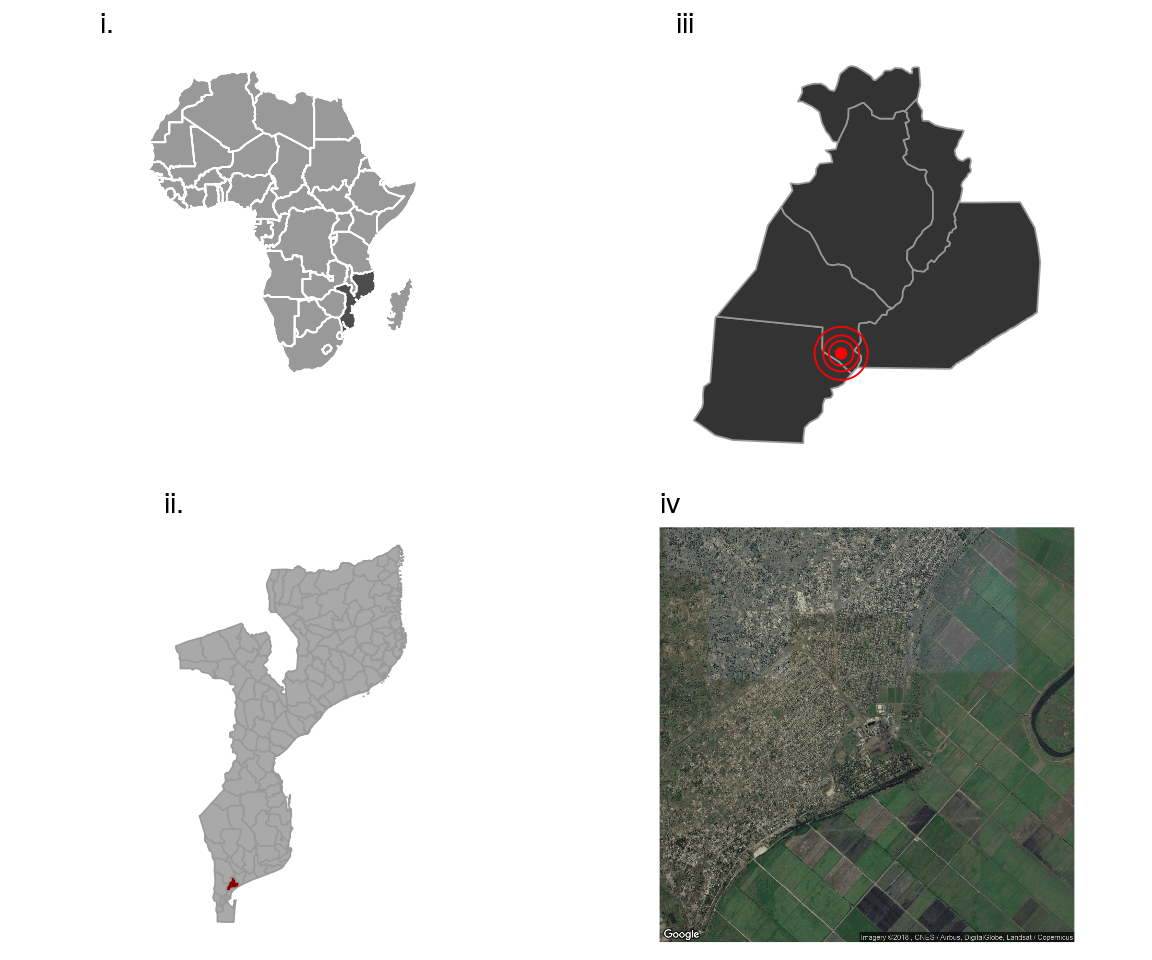
\includegraphics{figures/unnamed-chunk-14-1} 

}

\caption{(i) Mozambique in Africa, (ii) Districts of Mozambique with Manhiça highlighted in red, (iii) District of Manhiça with Maragra highlighted in red, (iv) Maragra SA with surrounding fields and village}\label{fig:unnamed-chunk-14}
\end{figure}

The mill of the Maragra Açucar SA (a subsidary of the Illovo sugar
company, henceforth referred to as ``Maragra'') was nationalized in the
1970s (like all other Mozambican mills), went through a period of low
production, and then fell completely out of use by 1984. It re-opened in
private hands in 1992, and was renovated by a group of international
investors in 1998. Today, Maragra accounts for roughly one quarter of
Mozambique's overall sugar production (second only to the nearby
Xinavane mill run by the Hulett Sugar Tongaat company) (Sutton, 2014).
With a favorably close location to the port of Maputo, ample land
(approximately 90 squared kilometers of plantation, and 5 squared
kilometers of factory grounds), approximately 5,000 employees (of which
three quarters are seasonal), and a mill with the capacity to process
not only all the sugarcane grown on Maragra's land, but also the cane of
the many nearby smallholders (O'Laughlin, 2016), Maragra has so far been
able to weather the 2016 Mozambican crisis and concurrent collapse in
global sugar prices.

Maragra (figure 1, panel iii) is located in the district of Manhiça
(figure 1, panel ii), a semi-rural area in the south of Mozambique
(figure 1, panel i). 80 kilometers north of the Mozambican capital of
Maputo, the district is low-lying, consisting largely of savannah and
wetlands along the Incomati River. Most of the areas 160,000 residents
(Sacoor et al., 2013) work as subsistence farmers. Migration from the
area to South Africa for the purpose of employment in the profitable
construction industry is common, especially among men (Nhacolo et al.,
2006), as is migration to the area (from other parts of Mozambique) for
seasonal work on the sugarcane plantations at Maragra and the slightly
larger facility in Xinavane (at the district's border with Magude)
(O'Laughlin, 2016).

Poverty is rife in southern Mozambique, and its associated illnesses
take their toll on the population. The community prevalence of HIV/AIDS
is as high as 40\% (González et al., 2012); even in a more recent study
suggesting a much lower prevalence of 22\%, the risk of infection is
still twice that of nearby areas (Mocumbi et al., 2017). Recent years
have seen a three-fold increase in tuberculosis (García-Basteiro et al.,
2017). Malaria, which has the greatest mortality burden due to the fact
that the young are especially vulnerable to its effects, is perennial,
though worse during the rainy season (December - March) (Saúte et al.,
2003). Adult malaria is essentially universal, albeit much of it
asymptomatic (Mayor et al., 2007). In regards to worker health, malaria
is Maragra's primary concern, being so important as to justify the
existence of both an on-site testing laboratory and clinic, as well as a
malaria control department.

Maragra workers are mostly seasonal, working for the firm approximately
half of the year during harvest time, and cultivating crops, working in
construction, or going unemployed (or working elsewhere) during the
other half. Though many workers live ``on-site'' (ie, within the
delineated property of the firm itself), a sizeable minority resides in
the environs (figure 1, panel iv). Maragra provides indoor residual
spraying (IRS) using ACT (alpha-cypermethrin) and DDT
(Dichlorodiphenyltrichloroethane) depending on stocks (a preference
apparently exists for the former, but it is not always available). IRS
activities, managed by Maragra's Malaria Control program, are ongoing
throughout the year (Figure 1, panel i). Nearly all on-site houses are
sprayed, though the time between fumigations is irregular (Figure 2,
panel ii). Off-site houses may also receive IRS (managed and carried out
by the National Malaria Control Program), but the status and timing of
these fumigations is not known at the individual level.

\begin{figure}[!h]

{\centering 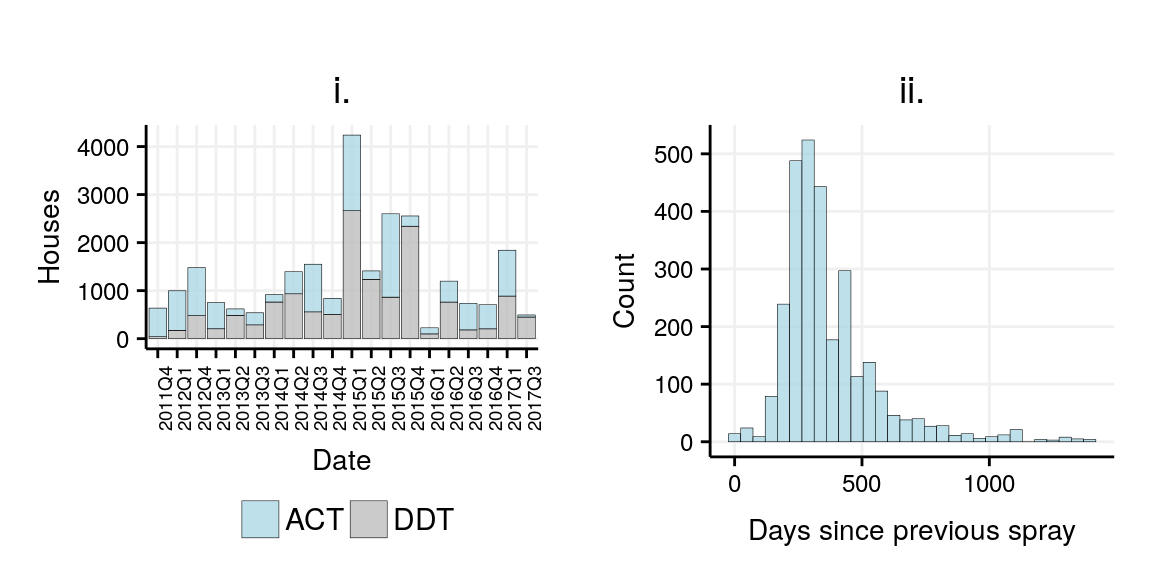
\includegraphics{figures/unnamed-chunk-16-1} 

}

\caption{i. Fumigation activities carried out by Maragra Malaria Control during study period, ii. Distribution of average time between sprayings of households}\label{fig:unnamed-chunk-16}
\end{figure}

\newpage

\section{Methods}\label{methods}

\subsection{Data}\label{data}

In collaboration with the sugar processing facility, we collected data
for the period from January 2010 through December 2016. Data came from
four sources: (i) the Human Resources' roster of worker details and
absences, (ii) the facility's on-site clinic's medical and laboratory
records, (iii) the facility's on-site malaria control program's records
pertaining to the dates, chemicals, and location of IRS activities, and
(iv) interviews with company employees pertaining to costs, data
limitations, etc. Digitization and collection of data took place during
the period from March 2016 through May 2017. Supplementary data
pertaining to worker characteristics was obtained from through the
Centro de Investigação em Saude de Manhiça's (CISM) demographic census,
which covered workers from the district, but not those who migrated from
other parts of the country (Nhacolo et al., 2006).

Data pertaining to district-wide malaria incidence was obtained from
Mozambique's Boletim Epidemiológico Semanal (BES), which is the system
by which the National Malaria Control Program monitors incidence at the
district level throghout the entire country, and reports the number of
confirmed weekly malaria cases at government health facilities. Using
these case numbers, combined with population estimates from the National
Statistical Institute (INE), we estimate each day's annualized weekly
malaria incidence rate (cases per 1000 population at risk), interpolated
from the weekly figures. We retrieved weather data for all Mozambican
stations from NOAA. We estimated the meteorological conditions at the
centroid of Manhiça using a simple interpolation method whereby the
district's weather conditions were estimated to be a function of all
Mozambican weather stations' reported conditions, inversely weighted by
kilometers from district centroid.

Maragra regularly employs IRS at on-site worker households in order to
reduce those workers' (and their families') risk of malaria infection.
IRS works by killing the malaria vector (mosquito), thereby preventing
infection of the household occupants. When administered correctly, IRS
is a low-risk intervention to its recipients, and is assumed not to
affect absenteeism in the short-term (to the extent that it may cause
negative side-effects, these are generally long-term). It is preventive
only, and does not cure current malaria infection, nor does it affect
the parasite load of mosquitoes. Workers living off-site (our control
group) also may have received IRS at some point during the study period
(from government programs). Even though we do not have reliable
person-level data on IRS carried out by the government, off-site workers
are a suitable control in the sense that they represent ``business as
usual'' (ie, what would happen if the company carried out no IRS and
relied solely on public interventions). Using company HR and clinical
records, we were able to identify absences and episodes of clinical
malaria among all workers, as well as identify the time since the most
recent IRS episode before the onsent of absence or illness.

Worker characteristics, illness and absenteeism data, along with IRS
activity data, were systematically stored, collected, and used at the
individual level by Maragra, and therefore of generally high quality.
Because cost data was less systematically collected by Maragra, and
because many costs could not be precisely quantified due to the
abundance of in-kind and cross-departmental expenditures, we had to rely
on rough estimations based on a mix of interviews, reciepts, and
interpolations. Since our program cost data is not as reliable as our
worker characteristic and outcome data, we were conservative in our
estimates, and generally tried to err on the side of program activities
and materials costing \emph{more} than what was reported, when doubt was
aired. Cost data consisted of three types: (i) wages of malaria control
employees, (ii) transporation and vehicle costs for IRS teams, and (iii)
acquisition costs of purchasing IRS chemicals for fumigation (ACT and
DDT), the latter two being combined into malaria control ``programme''
costs.

\subsection{Conceptual framework and identification
strategy}\label{conceptual-framework-and-identification-strategy}

We sought to understand the effect of IRS on individual workers'
likelihood of absence from work as well as their likelihood of clinical
malaria. To estimate this effect, we estimated separate models for
absence and illness. We employed linear mixed effects models (Minalu et
al., 2011) (Liu et al., 2010) (with individual worker fixed effects, and
random effects for other covariates) in lieu of interrupted time series
(Lopez Bernal et al., 2016) so as to explicitly adjust for confounders
(Bell and Jones, 2014). We divide into 4 different models for different
worker types, so as to account for the potential time-varying effects of
worker type on risk of malaria. Our model specification is as follows

\[
\hat{Y_{it}} = \hat{\beta}_{0} +  \hat{\beta}_{1}\text{Season}_{t} * (\hat{\beta}_2{IRS_{it}}*\hat{\beta}_3{IRStime_{it}}) + \alpha_i + \delta_t + \upsilon_{it}
\]

\(\hat{Y}_{it}\) is the rate of absence. \(\beta_{1}\) is the binary
``season'' variable, imputed from overall district clinical incidence.
Our intervention is whether the residence of the worker in question was
treated in the last year, and, if so, the time since treatment,
represented, respectively, by \(\beta_{2}\) and \(\beta_{3}\).
\(\alpha_i\) reprsents the time invariant worker fixed effects, and
\(\delta_i\) represents the fixed effect of the particular malaria
season. \(\upsilon\) is the error term.

We define the malaria season as any time during which the clinical
incidence of malaria in the district of Manhiça was at or greater than
the median clinical incidence of malaria for the entire study period.
These weeks are flagged as red in Figure 1, Panel A. By using clinical
incidence of the area of residence of the workers (as opposed to more
typical proxies for malaria risk, such as only rainy vs.~non rainy
season), our seasonality estimate is a closer approximation of true
malaria risk, incorporating lagged effects such as the incubation period
of the parasite, as well as any inherent non-linear effects of weather.
In addition, we adjust for daily precipitation; though its lagged effect
on malaria incidence is likely captured by the seasonality term, we
include rainfall since it's immediate effect (through its impact on
transportation and working conditions) may also affect absenteeism.

Details will go here about externalities (neighborhood effects, positive
spillover to district, negative spillover from district, how large firm
may mean that most positive externalities are absorbed by the firm, and
not many negative externalities, but maybe with a smaller firm it
wouldn't work as well)\todo{NOT DONE YET.}

\subsection{Estimating return on
investment}\label{estimating-return-on-investment}

Our formula for return on investment can be described in a
straightforward fashion\ldots{}

\begin{center}
$R = \dfrac{P_{w} - S_{wa} - S_{wc}}{P_{w}}$

\end{center}

\ldots{}where \(R\) is the return on investment, \(P\) is the malaria
control program's total operating cost, \(w\) refers to costs at the
per-worker level, \(a\) refers to savings through avoided absences, and
\$ c \$ refers to savings through avoided clinical encounters. We define
the malaria control program as ``profitable'' from an investment
standpoint if ROI is greater than 100\%, ie if the savings associated
with the estimated effect of IRS is greater than the costs of the
program's administration.

\subsection{Reproducibility and ethical
approval}\label{reproducibility-and-ethical-approval}

All data processing and analysis were carried out in R (R Core Team,
2017) and all analysis code is freely available online (Brew, 2017).
Ethical approval for this project was obtained from the Institutional
Ethics Review Board for Health at the CISM (CIBS-CISM) prior to data
collection.

\newpage

\section{Results}\label{results}

\subsection{Descriptive statistics}\label{descriptive-statistics}

We collected absenteeism and demographic data data on 3362 workers from
2012 through 2016. Workers were approximately 60\% male, and more than
80\% fieldworkers (predominantly cane-cutters). Most were in their 20s
and 30s and employed on temporary contracts. Table 1 shows overall
worker details divided by ``Treatment'' versus ``Control'' status.
``Treatment'' is considered the time beginning at IRS administration and
ending one year later; ``Control'' is considered time observed either
prior to IRS administration (and greater than 1 year after previous IRS
administration) or among workers who never received IRS. Because of the
temporal nature of these categories, many workers belong to both
treatment and control groups, albeit at different times.

\begin{table}[ht]
\centering
\begin{tabular}{rlllll}
  \hline
Variable &   & Treatment workers & Treatment days & Control workers & Control days \\ 
  \hline
Department & Administrative &  35 & 12523 & 157 & 173151 \\ 
   & Factory &  71 & 20533 & 453 & 280416 \\ 
   & Field & 410 & 91302 & 2691 & 1181175 \\ 
  Sex & F & 228 & 47907 & 1274 & 489484 \\ 
   & M & 288 & 76451 & 2027 & 1145258 \\ 
  Status & Permanent & 127 & 47075 & 500 & 655311 \\ 
   & Temporary & 389 & 77283 & 2801 & 979431 \\ 
  Age & 20 & 140 & 29463 & 960 & 347758 \\ 
   & 30 & 176 & 39119 & 1225 & 550783 \\ 
   & 40 & 123 & 30186 & 652 & 366936 \\ 
   & 50 &  58 & 18881 & 344 & 268877 \\ 
   & 60 &  17 & 5893 & 116 & 96555 \\ 
   & 70 &   2 & 816 &   4 & 3833 \\ 
   \hline
\end{tabular}
\caption{Overall worker characteristics} 
\end{table}

Temporary workers tended to be younger and male; female temporary
workers being on average 5-10 years older than their male counterparts.
Permanent workers had a bi-modal age distribution, the older peak
explained by the greater density of males in administrative roles.
Females accounted for 43\% of temporary workers but only 16\% of
permanent workers (figure x).

\begin{figure}[!h]

{\centering \includegraphics{figures/unnamed-chunk-19-1} 

}

\caption{Age distribution by sex and worker status}\label{fig:unnamed-chunk-19}
\end{figure}

During the study period, weather followed typical seasonal trends for
the area, albeit slightly drier than previous periods.

\begin{figure}[!h]

{\centering 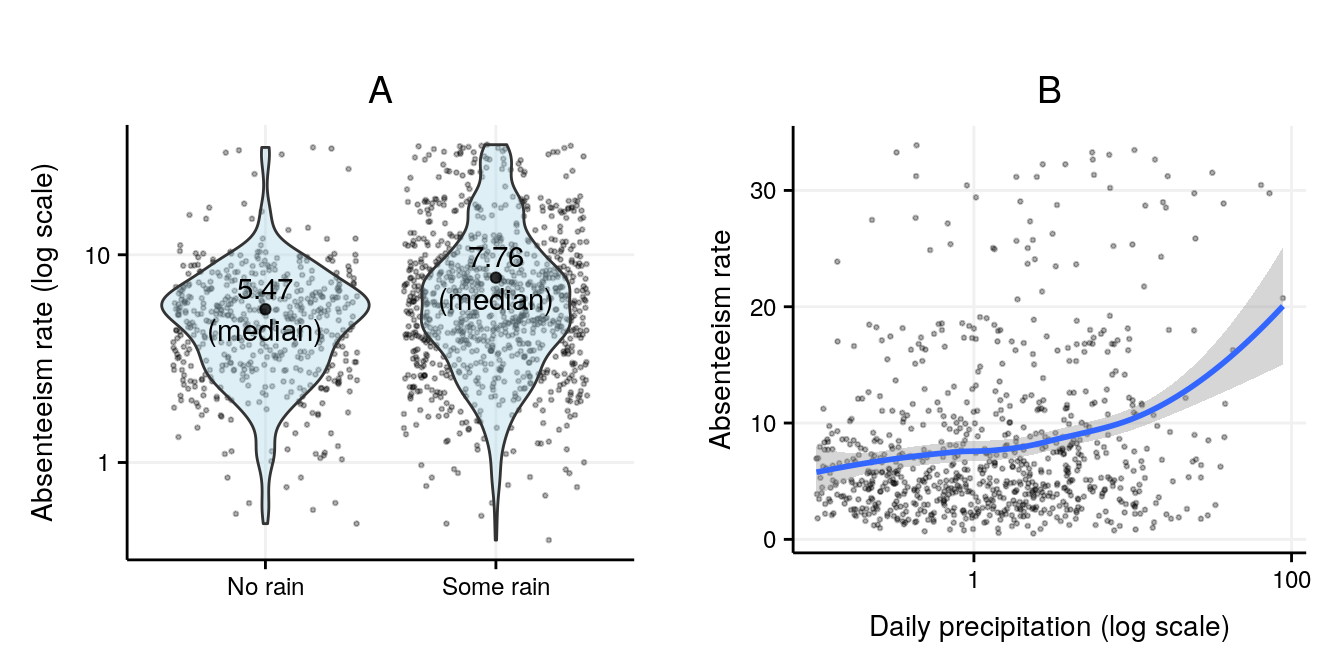
\includegraphics{figures/unnamed-chunk-20-1} 

}

\caption{i. Monthly total precipitation in the Maniça district; ii. Average monthly temperature (bars) during the study period, as well as monthly maximum (red) and minimum (blue) temperatures}\label{fig:unnamed-chunk-20}
\end{figure}

In Southern Mozambique, malaria peaks during the summer months (December
through March) most years (Figure 5, panel A), and worker absenteeism at
Maragra rates track malaria incidence closely, following the same
seasonal patterns (figure 4, panel B). Both all-cause absenteeism and
sick absenteeism have declined in recent years at Maragra (figure 5,
panel C), with the latter declining at a faster rate than the former.
The fact that the rate of confirmed cases at the company clinic is
largely non-seasonal (figure 5, panels E and F) suggests that a
significant portion of workers either seek care for malaria elsewhere
(for example, government health posts, of which several are nearby and
in some many cases closer to workers' residence than the company clinic)
or do not seek care during malaria infection. Accordingly, we focus our
analysis on all-cause absenteeism rather than sickness absenteeism or
malaria diagnostics, with the assumption that much of illness is
captured by absenteeism but not by the clinical data.

\begin{figure}
\centering
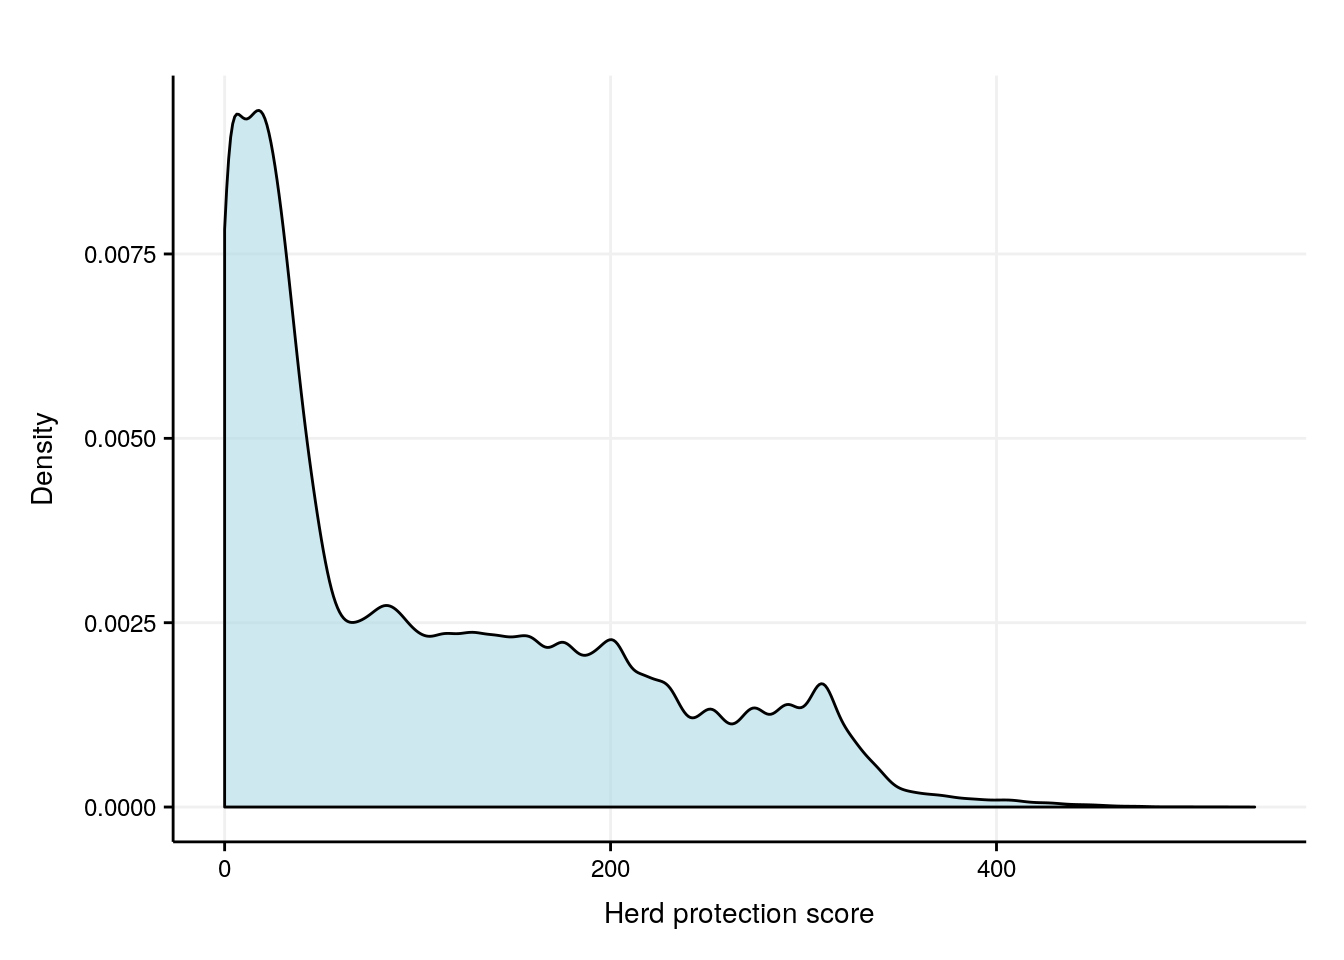
\includegraphics{figures/unnamed-chunk-21-1.pdf}
\caption{Clinical malaria (district of Manhiça), all-cause absenteeism
among Maragra workers, sick absenteeism among Maragra workers, positive
cases at company clinic, and test positivity rate at company clinic}
\end{figure}

\textbf{Fumigations}: During the period from January 1st, 2013 through
December 31st, 2016, the Maragra Malaria Control Unit carried out 11,007
episodes of fumigation of residential ``agregados'' (household
combinations), for a total of 13,260 building-fumigation combinations.
The total number of unique agregados sprayed during this period was
3,998. Among the 3,362 workers for whom we have reliable absenteeism and
residential data, 692 had their homes fumigated at least once (the
majority of workers live off of the facility).

\textbf{Absences}: We observed 1,759,100 unique worker-days among the
3,362 workers. The all-period average absenteeism rate was 5.56\%,
though this rate varied widely as a function of worker department, sex,
residence, and season (table 1).

\begin{table}[ht]
\centering
\begin{tabular}{rlllll}
  \hline
Variable &  & 2013 & 2014 & 2015 & 2016 \\ 
  \hline
Malaria season & Low & 5.2\% & 7\% & 5.4\% & 3.3\% \\ 
   & High & 8.2\% & 12.8\% & 6.3\% & 2.7\% \\ 
  Worker type & Field worker & 4.4\% & 7.6\% & 3.9\% & 1.7\% \\ 
   & Not field worker & 10.7\% & 12.4\% & 11.5\% & 9.6\% \\ 
  Contract & Permanent & 12.1\% & 12.6\% & 12\% & 10.2\% \\ 
   & Temporary & 0.1\% & 5\% & 2.3\% & 0.5\% \\ 
  Sex & F & 4\% & 8.1\% & 4.4\% & 1.9\% \\ 
   & M & 8.1\% & 10\% & 6.5\% & 3.7\% \\ 
  Residence & Off site & 6.4\% & 9.6\% & 5.9\% & 3\% \\ 
   & On site & 9.4\% & 9.7\% & 6.1\% & 3.1\% \\ 
  Precipitation & Dry & 5.4\% & 7.7\% & 4.8\% & 2.4\% \\ 
   & Rainy & 7.9\% & 10.6\% & 7\% & 3.3\% \\ 
   \hline
\end{tabular}
\caption{Absenteeism rate by year and worker characteristics} 
\end{table}

\textbf{Precipitation}: Of the 1454 days observed, 940 had no rainfall
at all (ie, approximately two-thirds). On days for which there was any
rainfall at all, the average amount was approximately 2.99 centimeters.
Rain was most common in December and January (average of 5-5.5 cm daily)
and least common in August and September (average of 0.5 cm daily). Days
with any rainfall saw more absenteeism than days with no rainfall
(Figure 6, panel A) and among days with any rainfall, more precipitation
was associated with greater absenteeism (Figure 6, panel B) (correlation
coefficient of 0.25).

\begin{figure}[!h]

{\centering 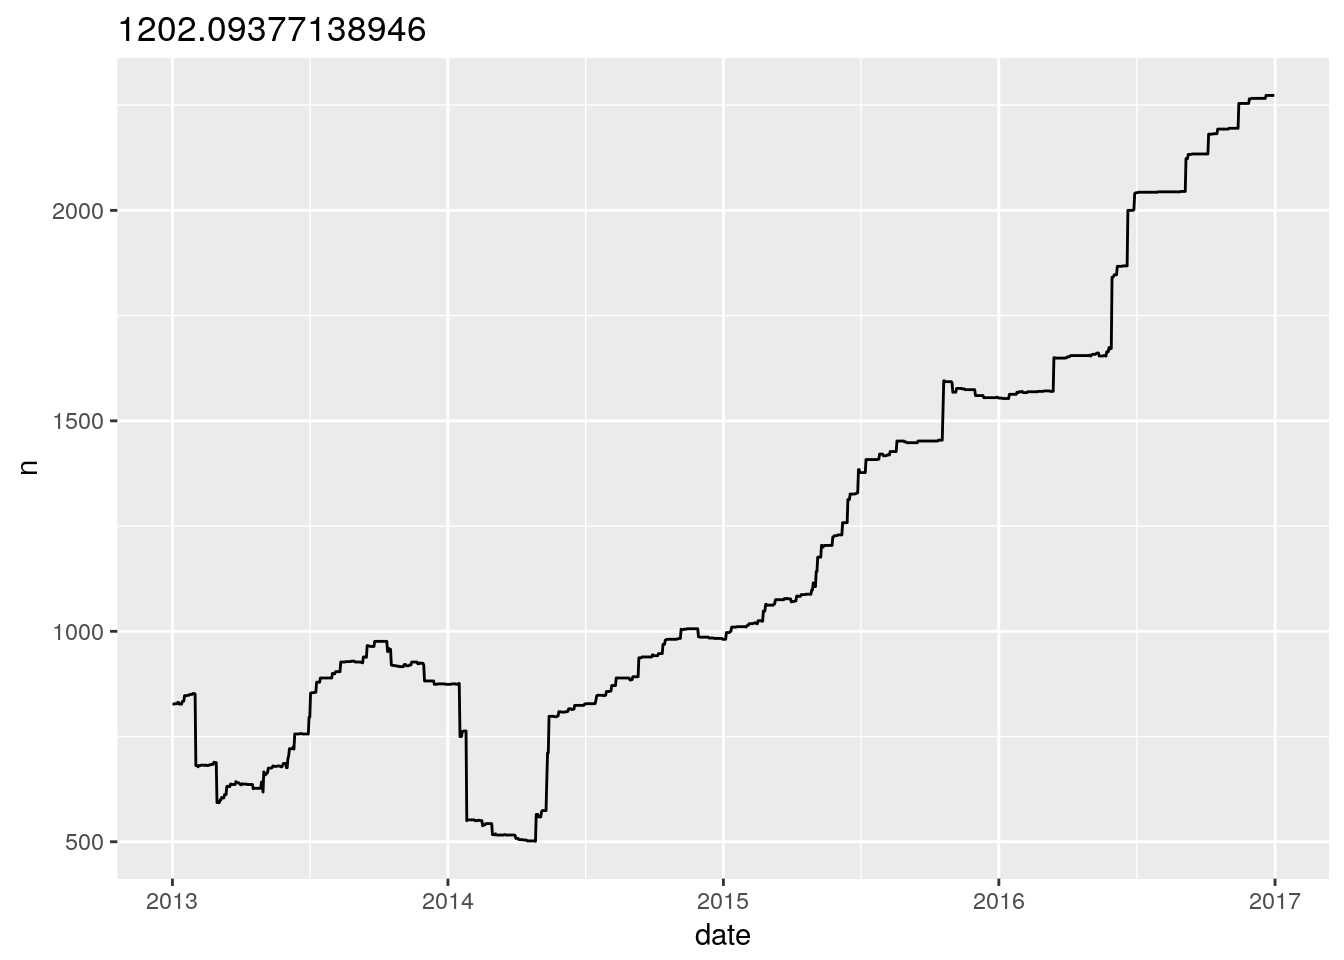
\includegraphics{figures/unnamed-chunk-26-1} 

}

\caption{Rainfall and absenteeism: association of any rainfall with absenteeism rate (left) and association of rainfall amount and absenteeism (right)}\label{fig:unnamed-chunk-26}
\end{figure}

The extent to which rainfall's effect on absenteeism is confounded by
its effect on malaria is discussed in the model results section.

\textbf{Effect of IRS on clinical malaria}: The number of malaria cases
registered at the company clinic during that time was 1873, for an
approximate annualized clinical incidence of 110 cases per 1,000.
\todo{Not done yet. In fact, not even sure if I should do this section at all, since it's basically just a distraction.}

\textbf{Costs of program}: The malaria control program at Maragra has an
annual operating budget of approximately \$112,000, which includes the
purchase of insecticide, the wages of IRS sprayers and drivers,
transportation, record-keeping, and general administrative costs.
Assuming linearity in costs, the program spends approximately \$19 per
building sprayed. With each agregado containing an average of 2.2
workers. Much of the benefit of IRS goes to non-worker residents of
sprayed agregados (who constitute a majority), but this benefit is
purposefully ignored for this analysis.

\textbf{Cost of malaria}: Given the likelihood that clinical data does
not fully capture all malaria cases (and most likely captures only a
small fraction of actual infections, given the high rates of acumulated
adult immunity {[}Mayor2007{]}), we do not quantify the costs of malaria
infection to the company. Rather, we first estimate the reduction in
absenteeism attributible to IRS, and then quantify the savings
associated with prevented absences. Additionally, we calculate the
clinical savings of IRS by first estimating the share of absences which
are associated with an episode of clinical malaria, and then applying
the clinical cost per case to the equivalent share of prevented
absences. We intentionally ignore the savings accrued by the public
health system, as well as the likely utility gains in secondary realms
such as school absenteeism, producitivity, etc.

\subsection{Analysis}\label{analysis}

\subsubsection{Effect of IRS on
absenteeism}\label{effect-of-irs-on-absenteeism}

Immediately following IRS, a worker's likelihood of absence drops
significantly (appendix figure, panel A). As one would expect if the
mechanism by which IRS reduces absence is through reduced malaria
infection, the effect of IRS during the low transmission season is
significant, but far less substantial in effect size (appendix figure,
panel B).

In order to assess the effect of IRS on absenteeism, we created 4 worker
fixed effects models for the 4 principal worker types (permanent field
worker, temporary field worker, permanent non-field worker, temporary
non-field worker) for both outcoms (all cause absenteeism vs.~sickness
absenteeism). The reason for segregating models rather than
incorporating worker type as a fixed effect was that it seemed plausible
that the effect of the treatment (IRS) on the outcome would be different
(and vary differently over time) depending on these worker types. For
instance, it is reasonable to assume that IRS' effect would be
differential for a temporary worker (who likely lives in the fumigated
house less than 100\% of the year) than for a permanent worker.

Given that IRS is carried out on a continuous rolling basis, we used
relative worker time (as opposed to calendar) as the time component of
our model - that is, each workers' days until and since IRS were
standardized so that day 0 (date of fumigation) was the interruption
point. This has the advantage of incorporating into the model a variety
of potential time-varying confounders in a quasi-randomized fashion,
thereby making it unecessary to adjust for them specifically. Our model
took into account workers' residential location (on or off site) - even
though off site workers by definition could not be administered IRS by
Maragra - so as to capture other seasonal effects from those workers.
\todo{This is not very eloquent yet and needs to be improved.}

The model results for all cause absenteeism (table 4) suggest a
significant decrease in absenteeism following the administration of IRS.
The effect is ambivalent among temporary workers, whereas among
permanent workers the administration of IRS decreases absenteeism betwen
2.5 and 8.4 percentage points in the 2-9 month following administration.
These effects are consistent with IRS decreasing absence through the
medium of malaria, since (a) the effect is not as strong in the first
month (potentially during the parasite incubation phase), the effect is
stronger on field workers (who are more socioeconomically the
demographic at greater risk of malaria than their administrative
counterparts), and the effect is ambivalent among temporary workers
(since the protective effect of IRS is only a function of the amount of
time that the worker spends in the fumigated house).

\begin{table}

\caption{\label{tab:unnamed-chunk-28}All cause absenteeism: model results}
\centering
\begin{tabular}[t]{ll}
\toprule
Term & Estimate\\
\midrule
\addlinespace[1.5em]
\multicolumn{2}{l}{\textbf{Permanent field worker}}\\
\hspace{1em}Malaria season & 2.533 (P<0.001)\\
\hspace{1em}Months since IRS: 01 & 5.382 (P<0.001)\\
\hspace{1em}Months since IRS: 02-04 & 4.747 (P<0.001)\\
\hspace{1em}Months since IRS: 05-09 & -2.669 (P<0.001)\\
\hspace{1em}Precipitation (mm) & 0.206 (P<0.001)\\
\hspace{1em}Malaria season:Months since IRS: 01 & -6.262 (P<0.001)\\
\hspace{1em}Malaria season:Months since IRS: 02-04 & -8.388 (P<0.001)\\
\hspace{1em}Malaria season:Months since IRS: 05-09 & -3.71 (P<0.001)\\
\addlinespace[1.5em]
\multicolumn{2}{l}{\textbf{Permanent not field worker}}\\
\hspace{1em}Malaria season & 0.957 (P<0.001)\\
\hspace{1em}Months since IRS: 01 & -0.987 (P=0.071)\\
\hspace{1em}Months since IRS: 02-04 & 4.375 (P<0.001)\\
\hspace{1em}Months since IRS: 05-09 & -0.55 (P=0.254)\\
\hspace{1em}Precipitation (mm) & 0.548 (P<0.001)\\
\hspace{1em}Malaria season:Months since IRS: 01 & 1.787 (P=0.016)\\
\hspace{1em}Malaria season:Months since IRS: 02-04 & -5.208 (P<0.001)\\
\hspace{1em}Malaria season:Months since IRS: 05-09 & -2.04 (P=0.003)\\
\addlinespace[1.5em]
\multicolumn{2}{l}{\textbf{Temporary field worker}}\\
\hspace{1em}Malaria season & -0.368 (P<0.001)\\
\hspace{1em}Months since IRS: 01 & -0.075 (P=0.526)\\
\hspace{1em}Months since IRS: 02-04 & -0.193 (P=0.072)\\
\hspace{1em}Months since IRS: 05-09 & -0.036 (P=0.738)\\
\hspace{1em}Precipitation (mm) & 0.02 (P<0.001)\\
\hspace{1em}Malaria season:Months since IRS: 01 & -0.154 (P=0.406)\\
\hspace{1em}Malaria season:Months since IRS: 02-04 & 0.297 (P=0.05)\\
\hspace{1em}Malaria season:Months since IRS: 05-09 & 0.041 (P=0.769)\\
\addlinespace[1.5em]
\multicolumn{2}{l}{\textbf{Temporary not field worker}}\\
\hspace{1em}Malaria season & 2.025 (P<0.001)\\
\hspace{1em}Months since IRS: 01 & -2.536 (P=0.134)\\
\hspace{1em}Months since IRS: 02-04 & -1.177 (P=0.282)\\
\hspace{1em}Months since IRS: 05-09 & -1.821 (P=0.084)\\
\hspace{1em}Precipitation (mm) & 0.078 (P<0.001)\\
\hspace{1em}Malaria season:Months since IRS: 01 & 6.121 (P=0.002)\\
\hspace{1em}Malaria season:Months since IRS: 02-04 & 1.333 (P=0.343)\\
\hspace{1em}Malaria season:Months since IRS: 05-09 & -4.639 (P<0.001)\\
\bottomrule
\end{tabular}
\end{table}

The model results for sickness only absenteeism (table 5) suggest that
IRS has a significant effect on permanent field workers. The effect is
directionally similar among temporary fieldworkers (but does not reach
the level of significance). Among non-fieldworkers, the effect of IRS is
mixed.

\begin{table}

\caption{\label{tab:unnamed-chunk-29}Sick absenteeism only: model results}
\centering
\begin{tabular}[t]{ll}
\toprule
Term & Estimate\\
\midrule
\addlinespace[1.5em]
\multicolumn{2}{l}{\textbf{Permanent field worker}}\\
\hspace{1em}Malaria season & -0.073 (P=0.089)\\
\hspace{1em}Months since IRS: 01 & 0.891 (P<0.001)\\
\hspace{1em}Months since IRS: 02-04 & 1.223 (P<0.001)\\
\hspace{1em}Months since IRS: 05-09 & -0.236 (P=0.249)\\
\hspace{1em}Precipitation (mm) & 0 (P=0.984)\\
\hspace{1em}Malaria season:Months since IRS: 01 & -1.501 (P<0.001)\\
\hspace{1em}Malaria season:Months since IRS: 02-04 & -0.597 (P=0.031)\\
\hspace{1em}Malaria season:Months since IRS: 05-09 & -0.484 (P=0.097)\\
\addlinespace[1.5em]
\multicolumn{2}{l}{\textbf{Permanent not field worker}}\\
\hspace{1em}Malaria season & -0.056 (P=0.204)\\
\hspace{1em}Months since IRS: 01 & -0.667 (P=0.003)\\
\hspace{1em}Months since IRS: 02-04 & 0.904 (P<0.001)\\
\hspace{1em}Months since IRS: 05-09 & 0.127 (P=0.526)\\
\hspace{1em}Precipitation (mm) & -0.002 (P=0.565)\\
\hspace{1em}Malaria season:Months since IRS: 01 & 1.121 (P<0.001)\\
\hspace{1em}Malaria season:Months since IRS: 02-04 & -0.122 (P=0.652)\\
\hspace{1em}Malaria season:Months since IRS: 05-09 & 1.198 (P<0.001)\\
\addlinespace[1.5em]
\multicolumn{2}{l}{\textbf{Temporary field worker}}\\
\hspace{1em}Malaria season & -0.106 (P<0.001)\\
\hspace{1em}Months since IRS: 01 & 0.029 (P=0.545)\\
\hspace{1em}Months since IRS: 02-04 & 0.04 (P=0.35)\\
\hspace{1em}Months since IRS: 05-09 & -0.046 (P=0.291)\\
\hspace{1em}Precipitation (mm) & 0 (P=0.966)\\
\hspace{1em}Malaria season:Months since IRS: 01 & -0.108 (P=0.148)\\
\hspace{1em}Malaria season:Months since IRS: 02-04 & -0.032 (P=0.595)\\
\hspace{1em}Malaria season:Months since IRS: 05-09 & -0.052 (P=0.36)\\
\addlinespace[1.5em]
\multicolumn{2}{l}{\textbf{Temporary not field worker}}\\
\hspace{1em}Malaria season & -0.135 (P=0.236)\\
\hspace{1em}Months since IRS: 01 & 1.427 (P=0.092)\\
\hspace{1em}Months since IRS: 02-04 & -0.569 (P=0.299)\\
\hspace{1em}Months since IRS: 05-09 & -1.42 (P=0.007)\\
\hspace{1em}Precipitation (mm) & -0.005 (P=0.613)\\
\hspace{1em}Malaria season:Months since IRS: 01 & -1.796 (P=0.069)\\
\hspace{1em}Malaria season:Months since IRS: 02-04 & 2.479 (P<0.001)\\
\hspace{1em}Malaria season:Months since IRS: 05-09 & 0.18 (P=0.794)\\
\bottomrule
\end{tabular}
\end{table}

\subsubsection{Externalities}\label{externalities}

This section is in progress. Looking at neighborhood effects,
core-periphery effects, etc.

\subsection{Translating absences to
costs}\label{translating-absences-to-costs}

xxx\todo{Not done yet. This will be relatively straightforward arithmetic, but I want to first make sure that the models are rock solid (since all of the "translation" hinges on them).}

\subsection{Return on investment}\label{return-on-investment}

\todo{Not done yet. In conversation with Eduardo from MC about getting more accurate costs}

\textbf{Savings}

\begin{itemize}
\tightlist
\item
  In percentage point terms, reduction from 13\% to 8\%.\\
\item
  5 annually prevented absences per worker.\\
\item
  8,000 workers: 40,000 prevented absences, wage of 3 USD
\item
  TOTAL: 120,000 USD in productivity-only savings.
\end{itemize}

\textbf{Costs}

\begin{itemize}
\tightlist
\item
  8 IRS workers, 1500 USD yearly = 12,000 USD\\
\item
  ACT + DDT: 50,000 USD
\item
  Facilities, vehicles, gas: 50,000 USD\\
\item
  TOTAL: 112,000 USD in IRS-only costs
\end{itemize}

\textbf{7\% ROI} (ignoring clinical costs)

\newpage

\subsection{Robustness and
generalizability}\label{robustness-and-generalizability}

Two principal concerns call into question the results of our analysis.
First, the application of IRS to a workers house may be
endogenous.\todo{Is this the right term here? We're not dealing with an "unobserved" factor per se, rather we're dealing with a situation in which the cause might influence the effect, and the effect might influence the cause, ie a feedback loop.}
It is reasonable to suspect that the application of IRS to households is
not random, but rather that IRS was applied more frequently to houses
which had already seen a malaria case. In this case, our estimated
effect of IRS on absenteeism would likely be underestimated, with the
post-IRS absenteeism rates actually having declined from a greater
pre-IRS absenteeism rate than otherwise suggested.

To check for this, we estimate the odds of absenteeism as a function of
receiving IRS \emph{during the 10 day period prior to receiving IRS}. If
IRS application is indeed endogenous, we would expect absenteeism to be
elevated during this period (since the increase in absenteeism would be
theoretically responsible for the application of IRS), a situation which
would require further statistical adjustment. If, on the other hand,
there is no endogeneity, we would expect absenteeism in the 10 day
period prior to IRS administration to be similar to other pre-IRS
absenteeism (adjusting for
seasonality).\todo{Should add model specification formula here.}

The below shows our robustness check for all cause absenteeism.

\begin{table}[H]
\centering
\begin{tabular}{l|r|r|r|r|l}
\hline
Variable & Estimate & Lower & Upper & P value & Significant\\
\hline
(Intercept) & 0.0661899 & 0.0614958 & 0.0711710 & 0.0000000 & xxx\\
\hline
\rowcolor{yellow}  10 days prior to IRS & 0.9229176 & 0.7300243 & 1.1503819 & 0.4886243\\
\hline
Malaria season & 3.1173457 & 2.9319429 & 3.3156586 & 0.0000000 & xxx\\
\hline
departmentFactory & 1.0944261 & 1.0118141 & 1.1841680 & 0.0245210 & x\\
\hline
departmentField & 0.5426841 & 0.5036184 & 0.5850353 & 0.0000000 & xxx\\
\hline
\rowcolor{yellow}  10 days prior to IRS:Malaria season & 0.8172244 & 0.6161822 & 1.0908542 & 0.1653822\\
\hline
\end{tabular}
\end{table}

The below shows our robustness check for sick only absenteeism. Unlike
with all cause absenteeism, during malaria season, being in the period
10 days prior to IRS is associated with statistically greater likelihood
of being absent for illness. In other words, it appears that there is
somewhat of a feedback loop: when a worker misses work due to illness,
his/her likelihood of getting IRS doubles in the next 10
days.\todo{What to do about this???}

\begin{table}[H]
\centering
\begin{tabular}{l|r|r|r|r|l}
\hline
Variable & Estimate & Lower & Upper & P value & Significant\\
\hline
(Intercept) & 0.0098162 & 0.0079914 & 0.0119339 & 0.0000000 & xxx\\
\hline
\rowcolor{yellow}  10 days prior to IRS & 0.6780540 & 0.3484288 & 1.1791509 & 0.2069281\\
\hline
Malaria season & 1.1637020 & 0.9827900 & 1.3767569 & 0.0777162 & \\
\hline
departmentFactory & 1.3068546 & 1.0428447 & 1.6460818 & 0.0214002 & x\\
\hline
departmentField & 0.6713828 & 0.5396839 & 0.8403182 & 0.0004142 & xxx\\
\hline
\rowcolor{yellow}  10 days prior to IRS:Malaria season & 2.2225088 & 1.0747201 & 4.8587934 & 0.0360020 & x\\
\hline
\end{tabular}
\end{table}

The second concern is that our quantification of return on investment is
distorted by the fact that we treat IRS operations as essentially linear
in nature, when in reality economies of scale, in-kind purchases and
other factors likely make the true cost-per-spraying convex. We address
this by creating three scenarios: (1) a ``start-up'' scenario in which
we take into account all costs incurred by starting a program from
scratch, (2) a ``normal'' scenario in which we match the assumptions
with those used in this paper (ie, account for ``wear-and-tear''
depreciation but not vehicle purchase, etc.) and a (3) ``absorbed
costs'' scenario which ignores all costs which are not directly incurred
by the program\ldots{}. xxx\ldots{}
\todo{Will address this with some sensitivity analysis}

\newpage

\section{Discussion}\label{discussion}

\todo{This entire section will not be done until methods/results are finalized.}

\begin{itemize}
\tightlist
\item
  Overview of findings
\item
  How this contributes to the literature
\item
  Implications for policy and for businesses
\item
  Spillover effects !
\item
  How absenteeism might be \emph{underestimating} true effect, since at
  the margin a sick worker might go to work (ie, not be absent), but be
  less productive
\end{itemize}

\subsection{Limitations}\label{limitations}

\begin{itemize}
\tightlist
\item
  No analysis yet of different worker types (agricultural
  vs.~industrial).
\item
  Have not yet ventured at all into side-analyses (effect on employment,
  tonnage, etc.).
\item
  Sick absenteeism seems to track absenteeism poorly: lack of clarity
  regarding pathways.
\item
  Large sample size, but all from same place: questionable
  generalizability.
\end{itemize}

\newpage

\section{Appendix}\label{appendix}

\subsection{Unadjusted absenteeism by time since
IRS}\label{unadjusted-absenteeism-by-time-since-irs}

\begin{figure}
\centering
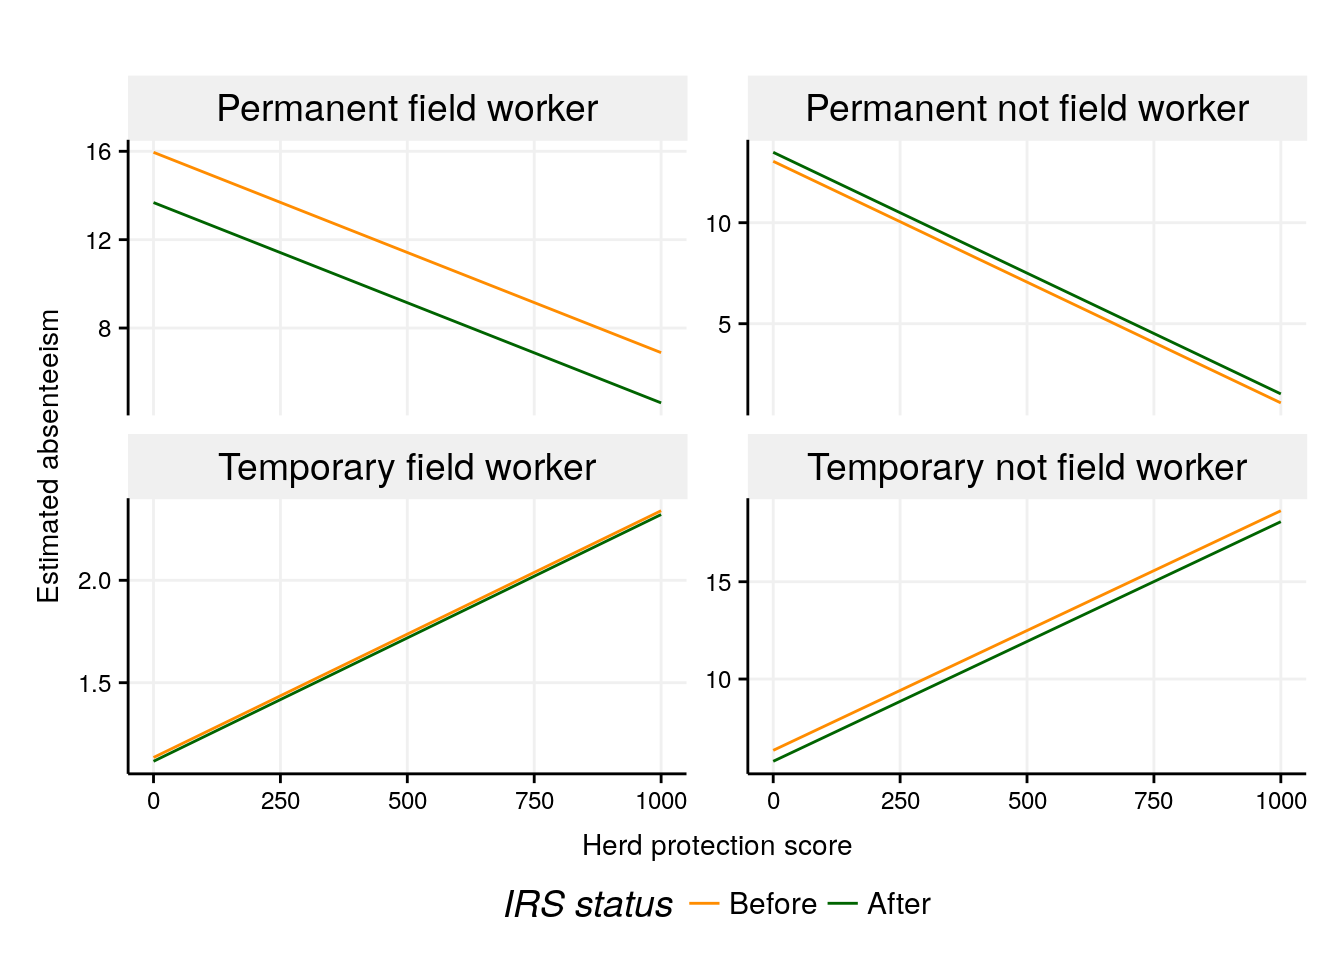
\includegraphics{figures/unnamed-chunk-33-1.pdf}
\caption{i. Absenteeism before and after IRS administration for all
workers who ever received IRS; ii. The same, but segregated by malaria
and non-malaria seasons}
\end{figure}

\subsection{Unadjusted sick absenteeism by time since
IRS}\label{unadjusted-sick-absenteeism-by-time-since-irs}

\begin{figure}
\centering
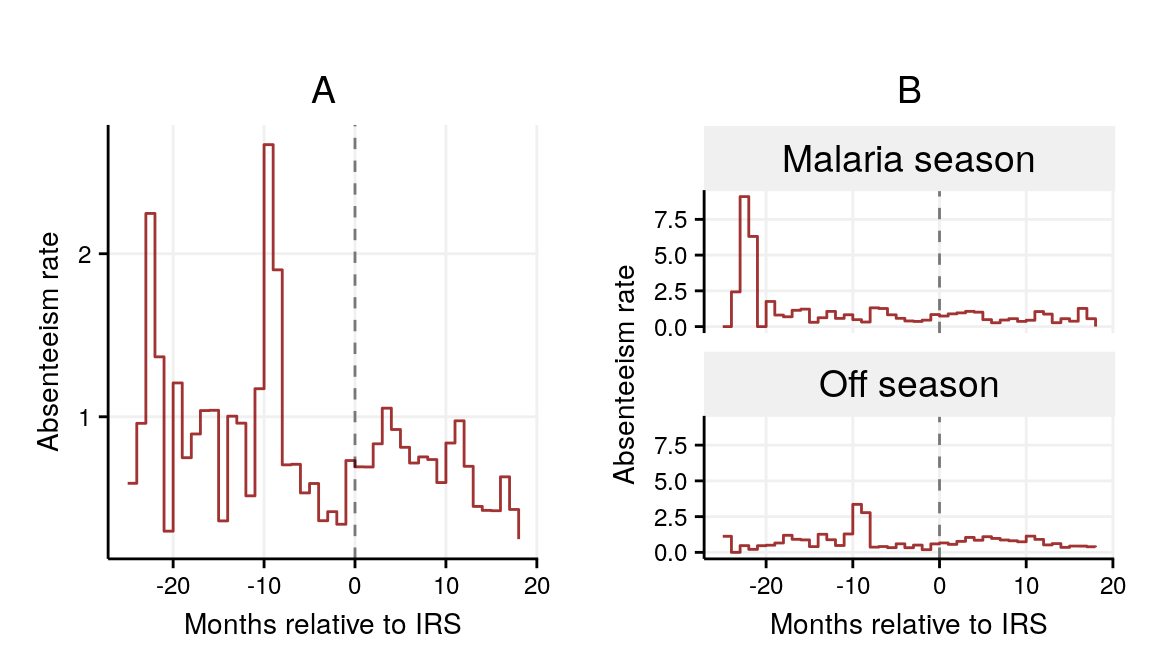
\includegraphics{figures/unnamed-chunk-34-1.pdf}
\caption{i. Sick absenteeism before and after IRS administration for all
workers who ever received IRS; ii. The same, but segregated by malaria
and non-malaria seasons}
\end{figure}

\section*{References}\label{references}
\addcontentsline{toc}{section}{References}

\hypertarget{refs}{}
\hypertarget{ref-Ajani2010}{}
Ajani, O., Ashagidigbi, W., 2010. Effect of malaria on rural households'
farm income in oyo state, nigeria. African Journal of Biomedical
Research 11. \url{https://doi.org/10.4314/ajbr.v11i3.50723}

\hypertarget{ref-AsensoOkyere1997}{}
Asenso-Okyere, W., Dzator, J.A., 1997. Household cost of seeking malaria
care. a retrospective study of two districts in ghana. Social Science \&
Medicine 45, 659--667.
\url{https://doi.org/10.1016/s0277-9536(96)00383-8}

\hypertarget{ref-Ashley2018}{}
Ashley, E.A., Phyo, A.P., Woodrow, C.J., 2018. Malaria. The Lancet.
\url{https://doi.org/10.1016/s0140-6736(18)30324-6}

\hypertarget{ref-asquino2015}{}
Asquino, M., 2016. Equatorial Guinea Plays a Leading Role in Combating
Malaria.

\hypertarget{ref-Azemar2009}{}
Azemar, C., Desbordes, R., 2009. Public governance, health and foreign
direct investment in sub-saharan africa. Journal of African Economies
18, 667--709. \url{https://doi.org/10.1093/jae/ejn028}

\hypertarget{ref-Bell2014}{}
Bell, A., Jones, K., 2014. Explaining fixed effects: Random effects
modeling of time-series cross-sectional and panel data. Political
Science Research and Methods 3, 133--153.
\url{https://doi.org/10.1017/psrm.2014.7}

\hypertarget{ref-Bennett_2017}{}
Bennett, A., Avanceña, A.L.V., Wegbreit, J., Cotter, C., Roberts, K.,
Gosling, R., 2017. Engaging the private sector in malaria surveillance:
A review of strategies and recommendations for elimination settings.
Malaria Journal 16. \url{https://doi.org/10.1186/s12936-017-1901-1}

\hypertarget{ref-Bloom2008}{}
Bloom, D., Canning, D., 2008. Population Health and Economic Growth
1--25.

\hypertarget{ref-brewgit}{}
Brew, J., 2017. Malaria and sugar: An in-depth examination of the effect
of malaria control activities on the health and productivity of maragra
sugarcane factory workers. GitHub repository.

\hypertarget{ref-World1999}{}
Brundtland, G.H., 1999. WHO on Health and Economic Productivity 25,
396--402.

\hypertarget{ref-Burton1999}{}
Burton, W.N., Conti, D.J., Chen, C.-Y., Schultz, A.B., Edington, D.W.,
1999. The role of health risk factors and disease on worker
productivity. Journal of Occupational \& Environmental Medicine 41,
863--877. \url{https://doi.org/10.1097/00043764-199910000-00007}

\hypertarget{ref-Buur2012}{}
Buur, L., Tembe, C.M., Baloi, O., 2012. The white gold: The role of
government and state in rehabilitating the sugar industry in mozambique.
Journal of Development Studies 48, 349--362.
\url{https://doi.org/10.1080/00220388.2011.635200}

\hypertarget{ref-CastelBranco2014}{}
Castel-Branco, C.N., 2014. Growth, capital accumulation and economic
porosity in mozambique: Social losses, private gains. Review of African
Political Economy 41, S26--S48.
\url{https://doi.org/10.1080/03056244.2014.976363}

\hypertarget{ref-anglo}{}
CCM, 2016. AngloGold Ashanti Malaria Control Ltd (AGA Mal).

\hypertarget{ref-Cole2006}{}
Cole, M.A., Neumayer, E., 2006. The impact of poor health on total
factor productivity. The Journal of Development Studies 42, 918--938.
\url{https://doi.org/10.1080/00220380600774681}

\hypertarget{ref-Curtis2003}{}
Curtis, C., Maxwell, C., Lemnge, M., Kilama, W., Steketee, R.W., Hawley,
W.A., Bergevin, Y., Campbell, C.C., Sachs, J., Teklehaimanot, A.,
Ochola, S., Guyatt, H., Snow, R.W., 2003. Scaling-up coverage with
insecticide-treated nets against malaria in africa: Who should pay? The
Lancet Infectious Diseases 3, 304--307.
\url{https://doi.org/10.1016/s1473-3099(03)00612-1}

\hypertarget{ref-Dillon2014}{}
Dillon, A., Friedman, J., Serneels, P., 2014. Health information,
treatment, and worker productivity: Experimental evidence from malaria
testing and treatment among nigerian sugarcane cutters. The World Bank.
\url{https://doi.org/10.1596/1813-9450-7120}

\hypertarget{ref-Dusfour2009}{}
Dusfour, I., Achee, N.L., Briceno, I., King, R., Grieco, J.P., 2009.
Comparative data on the insecticide resistance of anopheles~albimanus in
relation to agricultural practices in northern belize, CA. Journal of
Pest Science 83, 41--46. \url{https://doi.org/10.1007/s10340-009-0268-7}

\hypertarget{ref-lafarge}{}
Egedeye, L., Drozer, S., Leiser, A.-M., 2011. Corporate Action on
Malaria Control: Best Practices and Interventions.

\hypertarget{ref-Fink2015}{}
Fink, G., Masiye, F., 2015. Health and agricultural productivity:
Evidence from zambia. Journal of Health Economics 42, 151--164.
\url{https://doi.org/10.1016/j.jhealeco.2015.04.004}

\hypertarget{ref-GarcaBasteiro2017}{}
García-Basteiro, A.L., Ribeiro, R.M., Brew, J., Sacoor, C., Valencia,
S., Bulo, H., Cobelens, F., Macete, E., 2017. Tuberculosis on the rise
in southern mozambique (19972012). European Respiratory Journal 49,
1601683. \url{https://doi.org/10.1183/13993003.01683-2016}

\hypertarget{ref-German2013}{}
German, L., Schoneveld, G., Mwangi, E., 2013. Contemporary processes of
large-scale land acquisition in sub-saharan africa: Legal deficiency or
elite capture of the rule of law? World Development 48, 1--18.
\url{https://doi.org/10.1016/j.worlddev.2013.03.006}

\hypertarget{ref-Gonzlez2012}{}
González, R., Munguambe, K., Aponte, J., Bavo, C., Nhalungo, D., Macete,
E., Alonso, P., Menéndez, C., Naniche, D., 2012. High HIV prevalence in
a southern semi-rural area of mozambique: A community-based survey. HIV
Medicine 13, 581--588.
\url{https://doi.org/10.1111/j.1468-1293.2012.01018.x}

\hypertarget{ref-Goodman1999}{}
Goodman, C., Coleman, P., Mills, A., 1999. Cost-effectiveness of malaria
control in sub-saharan africa. The Lancet 354, 378--385.
\url{https://doi.org/10.1016/s0140-6736(99)02141-8}

\hypertarget{ref-Han}{}
Han, L., 2015. Malaria in Mozambique: trialling payment by results.

\hypertarget{ref-Hanson2004}{}
Hanson, K., 2004. Public and private roles in malaria control: The
contributions of economic analysis. The American Journal of Tropical
Medicine and Hygiene 71, 168--173.

\hypertarget{ref-Hong2011}{}
Hong, S.C., 2011. Malaria and economic productivity: A longitudinal
analysis of the american case. The Journal of Economic History 71,
654--671. \url{https://doi.org/10.1017/s0022050711001872}

\hypertarget{ref-Howard_2017}{}
Howard, N., Guinness, L., Rowland, M., Durrani, N., Hansen, K.S., 2017.
Cost-effectiveness of adding indoor residual spraying to case management
in afghan refugee settlements in northwest pakistan during a prolonged
malaria epidemic. PLOS Neglected Tropical Diseases 11, e0005935.
\url{https://doi.org/10.1371/journal.pntd.0005935}

\hypertarget{ref-Ijumba2002}{}
Ijumba, J.N., Mosha, F.W., Lindsay, S.W., 2002. Malaria transmission
risk variations derived from different agricultural practices in an
irrigated area of northern tanzania. Medical and Veterinary Entomology
16, 28--38. \url{https://doi.org/10.1046/j.0269-283x.2002.00337.x}

\hypertarget{ref-estatistica2009}{}
INE, 2011. Demographic health survey.

\hypertarget{ref-Jaleta2013}{}
Jaleta, K.T., Hill, S.R., Seyoum, E., Balkew, M., Gebre-Michael, T.,
Ignell, R., Tekie, H., 2013. Agro-ecosystems impact malaria prevalence:
Large-scale irrigation drives vector population in western ethiopia.
Malaria Journal 12, 350. \url{https://doi.org/10.1186/1475-2875-12-350}

\hypertarget{ref-Kaula_2017}{}
Kaula, H., Buyungo, P., Opigo, J., 2017. Private sector role, readiness
and performance for malaria case management in uganda, 2015. Malaria
Journal 16. \url{https://doi.org/10.1186/s12936-017-1824-x}

\hypertarget{ref-TheLancet2011}{}
Lancet, T., 2011. Malaria: Control vs elimination vs eradication. The
Lancet 378, 1117. \url{https://doi.org/10.1016/s0140-6736(11)61489-x}

\hypertarget{ref-Lee2017}{}
Lee, B.Y., Zenkov, E., Chatterjee, C., Candrinho, B., Zhang, S.,
Colborn, J., Briët, O.J.T., Brown, S.T., Mendis, C., Bartsch, S.M.,
Viisainen, K., DePasse, J.V., Stone, N.T.B., 2017. The economic value of
long-lasting insecticidal nets and indoor residual spraying
implementation in mozambique. The American Journal of Tropical Medicine
and Hygiene 96, 1430--1440. \url{https://doi.org/10.4269/ajtmh.16-0744}

\hypertarget{ref-Liu2010}{}
Liu, L., Strawderman, R.L., Cowen, M.E., Shih, Y.-C.T., 2010. A flexible
two-part random effects model for correlated medical costs. Journal of
Health Economics 29, 110--123.
\url{https://doi.org/10.1016/j.jhealeco.2009.11.010}

\hypertarget{ref-Lopez_Bernal_2016}{}
Lopez Bernal, J., Cummins, S., Gasparrini, A., 2016. Interrupted time
series regression for the evaluation of public health interventions: A
tutorial. International Journal of Epidemiology dyw098.
\url{https://doi.org/10.1093/ije/dyw098}

\hypertarget{ref-Mayor2007}{}
Mayor, A., Aponte, J.J., Fogg, C., Saúte, F., Greenwood, B., Dgedge, M.,
Menendez, C., Alonso, P.L., 2007.. Malaria Journal 6, 3.
\url{https://doi.org/10.1186/1475-2875-6-3}

\hypertarget{ref-McCarthy_2000}{}
McCarthy, D., Wolf, H., Wu, Y., 2000a. The growth costs of malaria.
\url{https://doi.org/10.3386/w7541}

\hypertarget{ref-McCarthy2000}{}
McCarthy, D., Wolf, H., Wu, Y., 2000b. The growth costs of malaria.
National Bureau of Economic Research.
\url{https://doi.org/10.3386/w7541}

\hypertarget{ref-Minalu2011}{}
Minalu, G., Aerts, M., Coenen, S., Versporten, A., Muller, A.,
Adriaenssens, N., Beutels, P., Molenberghs, G., Goossens, H., Hens, N.,
2011. Application of mixed-effects models to study the country-specific
outpatient antibiotic use in europe: A tutorial on longitudinal data
analysis. Journal of Antimicrobial Chemotherapy 66, vi79--vi87.
\url{https://doi.org/10.1093/jac/dkr460}

\hypertarget{ref-Mocumbi2017}{}
Mocumbi, S., Gafos, M., Munguambe, K., Goodall, R., and, S.M., 2017.
High HIV prevalence and incidence among women in southern mozambique:
Evidence from the MDP microbicide feasibility study. PLOS ONE 12,
e0173243. \url{https://doi.org/10.1371/journal.pone.0173243}

\hypertarget{ref-Moonasar_2016}{}
Moonasar, D., Maharaj, R., Kunene, S., Candrinho, B., Saute, F.,
Ntshalintshali, N., Morris, N., 2016. Towards malaria elimination in the
mosaswa (mozambique, south africa and swaziland) region. Malaria Journal
15. \url{https://doi.org/10.1186/s12936-016-1470-8}

\hypertarget{ref-Mouzin2011}{}
Mouzin, E., al., E., 2011. Business Investing in Malaria Control:
Economic Returns and a Healthy Workforce for Africa. Progress \& Impact
series.

\hypertarget{ref-Nhacolo_2006}{}
Nhacolo, A.Q., Nhalungo, D.A., Sacoor, C.N., Aponte, J.J., Thompson, R.,
Alonso, P., 2006. Levels and trends of demographic indices in southern
rural mozambique: Evidence from demographic surveillance in manhiça
district. BMC Public Health 6.
\url{https://doi.org/10.1186/1471-2458-6-291}

\hypertarget{ref-Nonvignon_2016}{}
Nonvignon, J., Aryeetey, G.C., Malm, K.L., Agyemang, S.A., Aubyn,
V.N.A., Peprah, N.Y., Bart-Plange, C.N., Aikins, M., 2016. Economic
burden of malaria on businesses in ghana: A case for private sector
investment in malaria control. Malaria Journal 15.
\url{https://doi.org/10.1186/s12936-016-1506-0}

\hypertarget{ref-Orem_2012}{}
Orem, J., Kirigia, J., Azairwe, R., Kasirye, I., Walker, O., 2012.
Impact of malaria morbidity on gross domestic product in uganda.
International Archives of Medicine 5, 12.
\url{https://doi.org/10.1186/1755-7682-5-12}

\hypertarget{ref-Overgaard2012}{}
Overgaard, H.J., Reddy, V.P., Abaga, S., Matias, A., Reddy, M.R.,
Kulkarni, V., Schwabe, C., Segura, L., Kleinschmidt, I., Slotman, M.A.,
2012. Malaria transmission after five years of vector control on bioko
island, equatorial guinea. Parasites \& Vectors 5, 253.
\url{https://doi.org/10.1186/1756-3305-5-253}

\hypertarget{ref-OLaughlin2016}{}
O'Laughlin, B., 2016. Consuming bodies: Health and work in the cane
fields in xinavane, mozambique. Journal of Southern African Studies 43,
625--641. \url{https://doi.org/10.1080/03057070.2016.1190519}

\hypertarget{ref-Phillips98}{}
Phillips, S.F.M., 1998. Economics and its contribution to the fight
against malaria. Annals of Tropical Medicine And Parasitology 92,
391--398. \url{https://doi.org/10.1080/00034989859375}

\hypertarget{ref-Pluess2009}{}
Pluess, B., Mueller, I., Levi, D., King, G., Smith, T.A., Lengeler, C.,
2009. Malaria a major health problem within an oil palm plantation
around popondetta, papua new guinea. Malaria Journal 8, 56.
\url{https://doi.org/10.1186/1475-2875-8-56}

\hypertarget{ref-Purdy_2013}{}
Purdy, M., Rublin, D., Wei, K., Robinson, M., 2013. The economic case
for combating malaria. The American Journal of Tropical Medicine and
Hygiene 89, 819--823. \url{https://doi.org/10.4269/ajtmh.12-0689}

\hypertarget{ref-R}{}
R Core Team, 2017. R: A language and environment for statistical
computing. R Foundation for Statistical Computing, Vienna, Austria.

\hypertarget{ref-Robbins2012}{}
Robbins, G., Perkins, D., 2012. Mining fdi and infrastructure
development on africa's east coast: Examining the recent experience of
tanzania and mozambique. Journal of International Development 24,
220--236. \url{https://doi.org/10.1002/jid.2817}

\hypertarget{ref-Sachs2002}{}
Sachs, J., Malaney, P., 2002. The economic and social burden of malaria.
Nature 415, 680--685. \url{https://doi.org/10.1038/415680a}

\hypertarget{ref-Sacoor2013}{}
Sacoor, C., Nhacolo, A., Nhalungo, D., Aponte, J.J., Bassat, Q.,
Augusto, O., Mandomando, I., Sacarlal, J., Lauchande, N., Sigauque, B.,
Alonso, P., Macete, E., 2013. Profile: Manhica health research centre
(manhica HDSS). International Journal of Epidemiology 42, 1309--1318.
\url{https://doi.org/10.1093/ije/dyt148}

\hypertarget{ref-Sate2003}{}
Saúte, F., Aponte, J., Ahmeda, J., Ascaso, C., Vaz, N., Dgedge, M.,
Alonso, P., 2003. Malaria in southern mozambique: Incidence of clinical
malaria in children living in a rural community in manhiça district.
Transactions of the Royal Society of Tropical Medicine and Hygiene 97,
655--660. \url{https://doi.org/10.1016/s0035-9203(03)80097-4}

\hypertarget{ref-Shretta2016}{}
Shretta, R., Avanceña, A.L.V., Hatefi, A., 2016. The economics of
malaria control and elimination: A systematic review. Malaria Journal
15. \url{https://doi.org/10.1186/s12936-016-1635-5}

\hypertarget{ref-Shretta_2017}{}
Shretta, R., Baral, R., Avanceña, A.L.V., Fox, K., Dannoruwa, A.P.,
Jayanetti, R., Jeyakumaran, A., Hasantha, R., Peris, L., Premaratne, R.,
2017. An investment case to prevent the reintroduction of malaria in sri
lanka. The American Journal of Tropical Medicine and Hygiene 16--0209.
\url{https://doi.org/10.4269/ajtmh.16-0209}

\hypertarget{ref-sutton}{}
Sutton, J., 2014. Mapa empresarial de moçambique.

\hypertarget{ref-Vecchi_2013}{}
Vecchi, V., Hellowell, M., Gatti, S., 2013. Does the private sector
receive an excessive return from investments in health care
infrastructure projects? Evidence from the uk. Health Policy 110,
243--270. \url{https://doi.org/10.1016/j.healthpol.2012.12.010}

\hypertarget{ref-White_2011}{}
White, M.T., Conteh, L., Cibulskis, R., Ghani, A.C., 2011. Costs and
cost-effectiveness of malaria control interventions - a systematic
review. Malaria Journal 10, 337.
\url{https://doi.org/10.1186/1475-2875-10-337}

\hypertarget{ref-White2014}{}
White, N.J., Pukrittayakamee, S., Hien, T.T., Faiz, M.A., Mokuolu, O.A.,
Dondorp, A.M., 2014. Malaria. The Lancet 383, 723--735.
\url{https://doi.org/10.1016/s0140-6736(13)60024-0}

\hypertarget{ref-World2016}{}
WHO, 2016. World Malaria Report.

\hypertarget{ref-whoprof}{}
WHO, 2015. Malaria profile: Mozambique.

\hypertarget{ref-Winkler}{}
Winkler, D., 2013. Potential and Actual FDI Spillovers in Global Value
Chains.

\hypertarget{ref-Wondwosen2018}{}
Wondwosen, B., Birgersson, G., Tekie, H., Torto, B., Ignell, R., Hill,
S.R., 2018. Sweet attraction: Sugarcane pollen-associated volatiles
attract gravid anopheles arabiensis. Malaria Journal 17.
\url{https://doi.org/10.1186/s12936-018-2245-1}


\end{document}
